% SyncBox manual - Firmware
% Written by Christopher Thomas.
%
% Copyright (c) 2021 by Vanderbilt University. This work is released under
% the Creative Commons Attribution-ShareAlike 4.0 International License.

\chapter{Firmware}
\label{sect-software}

The {\projectname} firmware consists of two polling loops that communicate 
via global variables. These are illustrated in Figure \ref{fig-firmware}.

\begin{figure}[h]
\begin{center}
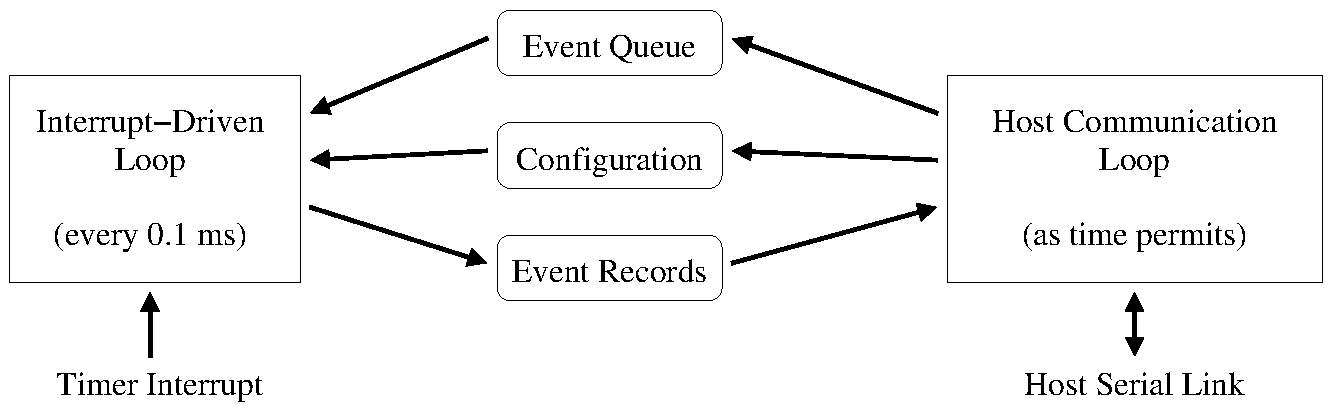
\includegraphics[width=0.9\columnwidth]{figs/firmware.pdf}
\end{center}
\caption{{\projectname} firmware block diagram.}\label{fig-firmware}
\end{figure}

The interrupt-driven loop is called at every measurement tick (0.1~ms 
intervals), and always occurs. During each loop, it sets output pin values 
as dictated by the event queue, and it attempts to read one analog input.

The host communication loop is called via the Arduino \texttt{loop()} 
function, and repeats as frequently as it can but with no time guarantees. 
During each loop, it polls the host serial link for inbound commands, 
queues events or alters internal state based on those commands, and 
reports events that have already occurred.

State information, including the event queue and records of events that 
have recently occurred, is stored in global variables. As these may be 
updated via interrupt service routines, they are flagged as 
\texttt{volatile} and are accessed from within \texttt{ATOMIC\_BLOCK()} 
constructs when read or modified by the host communication loop 
(interrupts are already atomic).

The following aspects of the firmware should be kept in mind:

\begin{itemize}
\item Analog reads take slightly longer than 0.1 millisecond. The 
interrupt-driven loop initiates conversions only when the analog to 
digital converter is not busy. With the default configuration, this means 
one conversion every 0.2 millisecond, or one full read of all analog 
inputs every 1.0 millisecond.

Analog inputs are read sequentially (round-robin order).

\item It is possible to set the reporting rate high enough that the serial 
link cannot keep up with the requested rate. What occurs in this scenario 
is that the host communication loop reports the \textit{most recent} set 
of events that occurred every time it is polled.

The result from the user's viewpoint is that records are silently dropped. 
This situation can be detected by paying close attention to the timestamps 
of reported events (these timestamps are always accurate).
\end{itemize}

%
% This is the end of the file.
